\chapter{單重態、貝爾不等式與不可克隆定理}

\lectureoverview{相對負號使原本僅具關聯的雙自旋態成為旋轉不變的單重態。我們藉由計算總自旋來辨認此態，利用其完全反相關來設計貝爾實驗，並將經典命題轉換為量子投影算符。由此得到的機率違反了經典的貝爾計數不等式。對定域性、實驗時序與不確定性的探問，接著引出線性量子力學的另一項推論：通用克隆機無法複製未知態。}

\section{一個符號能造成多大差別？}

考慮兩個電子，並在基底態中省略張量積符號：
\begin{equation}
  \ket{ud}\equiv\ket{u}_1\otimes\ket{d}_2,
  \qquad
  \ket{du}\equiv\ket{d}_1\otimes\ket{u}_2.
\end{equation}
有兩個特別簡單的疊加態，只差一個符號，
\begin{equation}
  \ket{\psi_\pm}
  =
  \frac{\ket{ud}\pm\ket{du}}{\sqrt2}.
  \label{eq:l05-two-signs}
\end{equation}
因子 \(1/\sqrt2\) 使總機率為一。在任一態中，沿第三軸測量都會得到相反的結果：若電子 1 的自旋向上，電子 2 的自旋就向下，反之亦然。因此，單靠這種關聯無法測出符號的差異。然而，這兩個態在物理上並不相同。

計算中會反覆用到泡利算符的作用：
\begin{align}
  \sigma_1\ket{u}&=\ket{d},&
  \sigma_1\ket{d}&=\ket{u},\nonumber\\
  \sigma_2\ket{u}&=i\ket{d},&
  \sigma_2\ket{d}&=-i\ket{u},\nonumber\\
  \sigma_3\ket{u}&=\ket{u},&
  \sigma_3\ket{d}&=-\ket{d}.
  \label{eq:l05-pauli-actions}
\end{align}
我們以 \(\sigma_i\) 表示作用於電子 1 的算符，並引入一組相同的算符 \(\tau_i\)，作用於電子 2。

\begin{figure}[htbp]
\centering
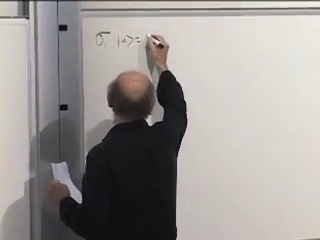
\includegraphics[width=0.62\linewidth]{lecture_05_figure_02.png}
\caption{比較中會用到的完整泡利算符作用表。}
\lectureframe{00:03:15}
\end{figure}

在這兩個態中，任一粒子的自旋都沒有偏好的方向：
\begin{equation}
  \expect{\sigma_i}_{\psi_\pm}=0,
  \qquad
  \expect{\tau_i}_{\psi_\pm}=0,
  \qquad i=1,2,3.
  \label{eq:l05-local-zero}
\end{equation}
例如，對加號態所要求的直接驗算如下：
\begin{align}
  \bra{\psi_+}\sigma_3\ket{\psi_+}
  &=
  \frac12
  \bigl(\bra{ud}+\bra{du}\bigr)
  \bigl(\ket{ud}-\ket{du}\bigr)\nonumber\\
  &=
  \frac12(1-1)=0.
  \label{eq:l05-sigma3-expectation}
\end{align}
交叉項會消失，因為 \(\braket{ud}{du}=0\)。

\begin{figure}[htbp]
\centering
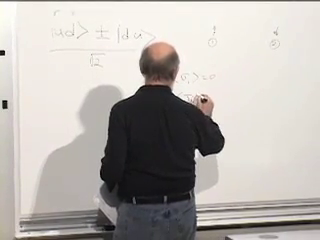
\includegraphics[width=0.78\linewidth]{lecture_05_figure_03.png}
\caption{加號態的期望值可藉由讓 \(\sigma_3\) 作用於態向量，再利用正交性求得。}
\lectureframe{00:07:00}
\end{figure}

\begin{classroomqa}
\lecturetimestamp{00:07:13}
\audiencequestion{期望值為零，是否表示測量單一自旋時會得到零？}
\lecturerresponse{不會。單一自旋分量的測量結果只有 \(+1\) 和 \(-1\)；\(\sigma_i\) 沒有零本徵值。方程~\eqref{eq:l05-local-zero}表示，重複測量的結果如同擲一枚公平的硬幣，而不是說任何一次測量結果為零。}
\end{classroomqa}

因此，第一個看似合理的判別方法行不通。局域平均值看不出相對符號，所以我們必須測量這對粒子的某種性質。

\section{總自旋選出單重態}

這對粒子的磁矩以向量和表示：
\begin{equation}
  \boldsymbol{\Sigma}
  =
  \boldsymbol{\sigma}+\boldsymbol{\tau}.
\end{equation}
總自旋的第三分量作用於兩個基底向量時都會給出零：
\begin{align}
  (\sigma_3+\tau_3)\ket{ud}
  &=(1-1)\ket{ud}=0,\nonumber\\
  (\sigma_3+\tau_3)\ket{du}
  &=(-1+1)\ket{du}=0.
\end{align}
因此，
\begin{equation}
  (\sigma_3+\tau_3)\ket{\psi_\pm}=0.
\end{equation}
兩種符號選擇在每一次測量中，總自旋的第三分量都是零。

第一分量則能區分兩者。由方程~\eqref{eq:l05-pauli-actions}可得：
\begin{align}
  (\sigma_1+\tau_1)\ket{ud}
  &=\ket{dd}+\ket{uu},\nonumber\\
  (\sigma_1+\tau_1)\ket{du}
  &=\ket{uu}+\ket{dd}.
\end{align}
因此，
\begin{align}
  (\sigma_1+\tau_1)\ket{\psi_+}
  &=
  \sqrt2\bigl(\ket{uu}+\ket{dd}\bigr),\nonumber\\
  (\sigma_1+\tau_1)\ket{\psi_-}
  &=0.
  \label{eq:l05-total-x}
\end{align}
加號態對這個可觀測量的期望值雖可能為零，卻不是其零本徵值所對應的本徵態。

\begin{classroomqa}
\lecturetimestamp{00:13:02}
\audiencequestion{若態向量不被算符作用成零，總自旋分量可能有哪些測量結果？}
\lecturerresponse{每個粒子的自旋分量測量結果為 \(+1\) 或 \(-1\)，所以兩者的和可能是 \(2\)、\(0\) 或 \(-2\)。期望值為零，並不表示每次測量結果都必定為零。}
\end{classroomqa}

第二分量完成了檢驗。在反對稱組合中，因子 \(i\) 會相消：
\begin{equation}
  (\sigma_2+\tau_2)\ket{\psi_-}=0.
\end{equation}
因此，三個分量都會將減號態作用成零：
\begin{equation}
  \bigl(\boldsymbol{\sigma}+\boldsymbol{\tau}\bigr)
  \cdot\hat n\,\ket{\psi_-}=0
  \qquad\text{for every unit vector }\hat n.
  \label{eq:l05-singlet-any-axis}
\end{equation}

\begin{figure}[htbp]
\centering
\includegraphics[width=0.84\linewidth]{lecture_05_figure_06.png}
\caption{逐一計算各分量時，項目相消，因而確認減號態的總自旋為零。}
\lectureframe{00:16:30}
\end{figure}

反對稱態 \(\ket{\psi_-}\) 是\emph{單重態}。它具有旋轉不變性：沿任何軸測量，總自旋的結果都相同，皆為零。方程~\eqref{eq:l05-two-signs}中的對稱態則屬於三重態子空間。

\begin{classroomqa}
\lecturetimestamp{00:19:06}
\audiencequestion{反向自旋的結果只在平均意義下成立嗎？}
\lecturerresponse{對單重態而言，每次測量都成立。方程~\eqref{eq:l05-singlet-any-axis}是本徵向量方程，因此在兩個粒子上沿同一軸測量自旋分量時，所得結果的總和必定等於本徵值零。}
\end{classroomqa}

\begin{classroomqa}
\lecturetimestamp{00:19:36}
\audiencequestion{為什麼另一個態稱為三重態？}
\lecturerresponse{這個名稱來自總自旋為一的多重態中有三個態。此處暫不推導；目前只需看出對稱態與一維單重態子空間之間的差別。}
\end{classroomqa}

如果 Bob 測量自己電子的任一自旋分量，他立刻就能知道 Alice 若測量自己電子的同一分量會得到什麼結果：她的結果必定相反。這是一種 Einstein--Podolsky--Rosen 關聯。一對暗中預設結果相反的硬幣，也能呈現相反結果，但只能對應一個預先安排好的問題。單重態則不論選擇哪一條空間軸，都呈現完全反相關。

\begin{classroomqa}
\lecturetimestamp{00:20:55}
\audiencequestion{糾纏是 Einstein、Podolsky 和 Rosen 最先發現的嗎？}
\lecturerresponse{不是。Schrödinger 曾討論這種現象，並引入「糾纏」一詞。EPR 論證則使遠距離關聯問題變得格外尖銳。}
\end{classroomqa}

\begin{classroomqa}
\lecturetimestamp{00:23:50}
\audiencequestion{這種即時關聯會違反因果律嗎？由哪位觀察者先測量，是否有影響？}
\lecturerresponse{這不會傳送任何可用來傳訊的資訊。無論 Bob 是否測量，在任何慣性參考系中，不論測量先後次序如何，Alice 的局域測量結果仍各有一半機率。她只有在透過一般的經典通道收到 Bob 的結果後，才能驗證兩者的關聯；這種通道傳遞資訊的速度不可能超過光速。}
\end{classroomqa}

\section{貝爾不等式是經典計數的結果}

貝爾結果的重要性有時讓人難以定論。有時它似乎是量子力學最深刻的特徵，有時又像是形式體系中另一個不可避免的推論。Bell 本人和 Feynman 也都曾表達這兩種看法。然而，不等式本身很簡單；令人意外的是它遭到違反。

取一組普通物件。每個物件可能具有或不具有三種性質 \(A\)、\(B\) 和 \(C\)。令 \(N(A,\neg B)\) 表示具有 \(A\)、但不具有 \(B\) 的物件數目。經典集合邏輯可推出
\begin{equation}
  N(A,\neg B)+N(B,\neg C)
  \geq
  N(A,\neg C).
  \label{eq:l05-bell-count}
\end{equation}
證明依據的是集合包含關係：
\begin{equation}
  A\cap C^{c}
  \subseteq
  (A\cap B^{c})\cup(B\cap C^{c}).
  \label{eq:l05-set-inclusion}
\end{equation}
確實，\(A\cap C^c\)中的元素不是屬於 \(B\)，就是不屬於它。若屬於，就屬於 \(B\cap C^c\)；若不屬於，就屬於 \(A\cap B^c\)。計算並集中的元素數目，只可能比左側集合中的元素數目多。

\begin{figure}[htbp]
\centering
\includegraphics[width=0.78\linewidth]{lecture_05_figure_07.png}
\caption{黑板上的證明將三個彼此重疊的經典子集劃分成若干非負區域。}
\lectureframe{00:31:15}
\end{figure}

同樣也可以用非負整數 \(N_i\)，標示三集合圖中互不重疊的區域。方程~\eqref{eq:l05-bell-count}兩側都包含 \(A\cap C^c\)所涵蓋的區域，而左側還多出一些非負區域。這裡沒有用到任何量子概念。這只是一個關於子集與一般邏輯選項的定理。

\section{將集合論陳述轉化為自旋實驗}

製備許多處於單重態的獨立電子對，並定義三個關於電子 1 的命題：
\begin{align}
  A&:\ \text{spin 1 is up at }0^\circ\text{, along the third axis},\nonumber\\
  B&:\ \text{spin 1 is up at }45^\circ\text{ in the }zx\text{-plane},\nonumber\\
  C&:\ \text{spin 1 is up at }90^\circ\text{, along the first axis}.
  \label{eq:l05-abc}
\end{align}

\begin{figure}[htbp]
\centering
\includegraphics[width=0.82\linewidth]{lecture_05_figure_08.png}
\caption{這三個自旋命題分別設定在同一平面中的 \(0^\circ\)、\(45^\circ\) 和 \(90^\circ\) 方向。}
\lectureframe{00:39:00}
\end{figure}

在單重態中，關於電子 1 的命題之否定，可以改寫為關於電子 2 的肯定命題。例如，
\begin{align}
  \neg B
  &:\ \text{spin 1 is down at }45^\circ\nonumber\\
  &\Longleftrightarrow
  \text{spin 2 is up at }45^\circ.
\end{align}
同樣地，\(\neg C\)可改寫為電子 2 沿 \(90^\circ\) 方向的自旋向上。

\begin{classroomqa}
\lecturetimestamp{00:40:04}
\audiencequestion{\(\neg C\)是否表示電子2沿\(90^\circ\)方向的自旋向下？}
\lecturerresponse{不是。先否定\(C\)：電子1沿\(90^\circ\)方向的自旋向下。再根據單重態的完全反相關，電子2沿同一軸的自旋便向上。這兩次反轉必須分開處理。}
\end{classroomqa}

對大量製備的電子對而言，計數與機率只差一個共同因子，也就是製備的電子對總數。旋轉不變性還給出
\begin{equation}
  P(A,\neg B)=P(B,\neg C),
\end{equation}
這是因為第二個實驗是將第一個實驗旋轉 \(45^\circ\) 的結果。因此，經典的貝爾不等式會要求
\begin{equation}
  2P(A,\neg B)\geq P(A,\neg C).
  \label{eq:l05-bell-probability}
\end{equation}
接著需要找出有效計算這些機率的方法。

\section{將命題表示為投影算符}

在一般的三維向量空間中，投影算符會去除向量中垂直於所選子空間的分量。一維投影算符將向量正交投影到一條直線上；二維投影算符則將它投影到一個平面上。若 \(P\) 是投影到指定子空間的投影算符，則
\begin{equation}
  P\ket{\alpha}=\ket{\alpha_P}.
\end{equation}

\begin{figure}[htbp]
\centering
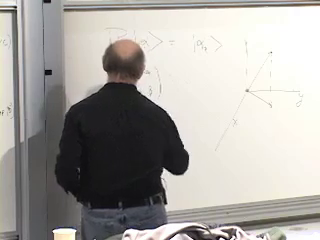
\includegraphics[width=0.76\linewidth]{lecture_05_figure_04.png}
\caption{圖中並列呈現幾何投影及其算符表示法。}
\lectureframe{00:49:53}
\end{figure}

\begin{figure}[htbp]
\centering
\begin{tikzpicture}[scale=1.05,>=Latex]
  \draw[->] (-0.25,0)--(4.0,0);
  \draw[thick] (-0.25,-0.25)--(3.55,2.6);
  \draw[->,very thick] (0,0)--(2.25,3.05)
    node[above] {\(\ket{\alpha}\)};
  \coordinate (P) at (2.72,1.98);
  \draw[dashed] (2.25,3.05)--(P);
  \draw[->,very thick] (0,0)--(P)
    node[right] {\(\ket{\alpha_P}\)};
  \node[below right] at (3.1,2.25) {projected subspace};
\end{tikzpicture}
\caption{重新繪製的投影幾何圖。}
\end{figure}

在單自旋希爾伯特空間中，命題 \(\sigma_3=+1\) 對應於由 \(\ket{u}\) 張成的一維子空間。其投影算符的作用為
\begin{equation}
  P_{\sigma_3=+1}
  \begin{pmatrix}\alpha\\\beta\end{pmatrix}
  =
  \begin{pmatrix}\alpha\\0\end{pmatrix},
  \qquad
  P_{\sigma_3=-1}
  \begin{pmatrix}\alpha\\\beta\end{pmatrix}
  =
  \begin{pmatrix}0\\\beta\end{pmatrix}.
  \label{eq:l05-projector-actions}
\end{equation}

\begin{classroomqa}
\lecturetimestamp{00:49:55}
\audiencequestion{第一個投影算符是否表示向量在垂直軸上有多高？}
\lecturerresponse{不是。它只是捨棄正交分量的係數 \(\beta\)。這些分量是希爾伯特空間中的振幅，不是自旋在一般空間中的座標。}
\end{classroomqa}

\begin{figure}[htbp]
\centering
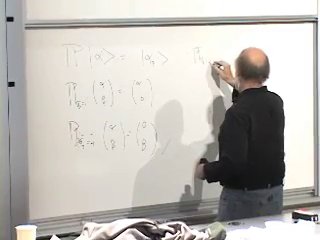
\includegraphics[width=0.78\linewidth]{lecture_05_figure_05.png}
\caption{先讓投影算符作用於一般旋量，再將它們寫成明確的矩陣形式。}
\lectureframe{00:51:40}
\end{figure}

矩陣形式為
\begin{equation}
  P_{\sigma_3=+1}
  =
  \begin{pmatrix}1&0\\0&0\end{pmatrix}
  =
  \frac{I+\sigma_3}{2}.
  \label{eq:l05-p3}
\end{equation}
沿任意單位向量 \(\hat n\) 方向，也可以用相同方式構造投影算符：
\begin{equation}
  P_{\boldsymbol{\sigma}\cdot\hat n=+1}
  =
  \frac{I+\boldsymbol{\sigma}\cdot\hat n}{2}.
  \label{eq:l05-pn}
\end{equation}

\begin{classroomqa}
\lecturetimestamp{00:53:09}
\audiencequestion{投影到 \(\sigma_1=+1\) 的投影算符是什麼？}
\lecturerresponse{在方程~\eqref{eq:l05-p3}中以\(\sigma_1\)取代\(\sigma_3\)：\(P_{\sigma_1=+1}=(I+\sigma_1)/2\)。}
\end{classroomqa}

現在可以用一種實用的命題形式來表達玻恩規則：
\begin{equation}
  P(\mathcal A\text{ is true in }\ket{\psi})
  =
  \bra{\psi}P_{\mathcal A}\ket{\psi}.
  \label{eq:l05-projector-born}
\end{equation}
對於歸一化旋量 \(\ket{\psi}=(\alpha,\beta)^T\)，在方程~\eqref{eq:l05-projector-born}中令 \(P_{\sigma_3=+1}\)，會得到 \(|\alpha|^2\)，正如預期。

這種表述凸顯了經典命題與量子命題的差異。在經典邏輯中，一個性質對應於集合的子集；在量子力學中，一個性質對應於希爾伯特空間的子空間，或等價地，對應於該子空間的投影算符。子集與向量子空間的格運算並不相同；貝爾矛盾的根源就在這個差異。

\subsection{貝爾聯合投影算符}

對於\(A\wedge\neg B\)，電子1必須沿第三軸自旋向上，而電子2必須沿著下列方向自旋向上：
\begin{equation}
  \hat n_{45}=\frac{\hat x+\hat z}{\sqrt2}.
\end{equation}
第二個自旋沿該方向的分量為
\begin{equation}
  \boldsymbol{\tau}\cdot\hat n_{45}
  =
  \frac{\tau_1+\tau_3}{\sqrt2}.
\end{equation}
因此，聯合投影算符為
\begin{equation}
  P_{A\wedge\neg B}
  =
  \frac{I+\sigma_3}{2}
  \frac{I+(\tau_1+\tau_3)/\sqrt2}{2}.
  \label{eq:l05-joint-projector}
\end{equation}

\begin{classroomqa}
\lecturetimestamp{00:59:18}
\audiencequestion{為什麼\(45^\circ\)方向的自旋分量中會有因子\(1/\sqrt2\)？}
\lecturerresponse{該方向向量必須是單位向量。它在第一軸和第三軸方向的分量都是\(1/\sqrt2\)，所以相應的可觀測量為\((\tau_1+\tau_3)/\sqrt2\)。}
\end{classroomqa}

\begin{classroomqa}
\lecturetimestamp{01:00:52}
\audiencequestion{整個表示式\(I+\boldsymbol{\tau}\cdot\hat n_{45}\)都要除以二嗎？}
\lecturerresponse{是。投影算符為\(\bigl(I+\boldsymbol{\tau}\cdot\hat n_{45}\bigr)/2\)；因子\(1/2\)乘在整個分子上。}
\end{classroomqa}

方程~\eqref{eq:l05-joint-projector}中的兩個因子作用於不同的張量因子，因此彼此對易。兩者依序作用時，先去掉電子1自旋向下的所有分量，再從留下的分量中去掉電子2沿\(\hat n_{45}\)方向自旋向下的部分。

\section{量子數值使不等式反轉}

令
\begin{equation}
  \ket{\psi_s}
  =
  \frac{\ket{ud}-\ket{du}}{\sqrt2}
\end{equation}
表示單重態。從下式開始：
\begin{equation}
  P(A,\neg B)
  =
  \bra{\psi_s}P_{A\wedge\neg B}\ket{\psi_s}.
\end{equation}
因子\((I+\sigma_3)/2\)會將\(\ket{du}\)作用成零，並留下\(\ket{ud}/\sqrt2\)。接著，第二個因子給出
\begin{align}
  \frac{I+(\tau_1+\tau_3)/\sqrt2}{2}\ket{ud}
  &\notag\\[-0.3em]
  &=
  \frac12
  \left[
    \ket{ud}
    +\frac{\ket{uu}-\ket{ud}}{\sqrt2}
  \right]\nonumber\\
  &=
  \frac12
  \Biggl[
    \left(1-\frac1{\sqrt2}\right)\ket{ud}
  \nonumber\\
  &\qquad
    +\frac1{\sqrt2}\ket{uu}\Biggr].
  \label{eq:l05-projector-action}
\end{align}
其中的 \(\ket{uu}\) 項與單重態的左矢正交，因此重疊為零；其餘歸一化因子給出
\begin{equation}
  P(A,\neg B)
  =
  \frac14\left(1-\frac1{\sqrt2}\right).
  \label{eq:l05-pab}
\end{equation}

\begin{figure}[htbp]
\centering
\includegraphics[width=0.88\linewidth]{lecture_05_figure_09.png}
\caption{投影算符計算中，保留了\(\ket{ud}\)的重疊，並捨棄正交的\(\ket{uu}\)項。}
\lectureframe{01:08:20}
\end{figure}

由旋轉不變性，下一組方向也會得到相同結果：
\begin{equation}
  P(B,\neg C)
  =
  \frac14\left(1-\frac1{\sqrt2}\right).
\end{equation}
對於\(A\wedge\neg C\)，第二個方向就是第一空間軸，因此
\begin{equation}
  P_{A\wedge\neg C}
  =
  \frac{I+\sigma_3}{2}\frac{I+\tau_1}{2}.
\end{equation}
第一個因子再次留下 \(\ket{ud}/\sqrt2\)。\(\tau_1\)項會產生\(\ket{uu}\)，與單重態的左矢正交；恆等算符項則會保留下來。因此，
\begin{equation}
  P(A,\neg C)=\frac14.
  \label{eq:l05-pac}
\end{equation}
合併這三個結果，
\begin{equation}
  \underbrace{
  P(A,\neg B)+P(B,\neg C)
  }_{\frac12(1-1/\sqrt2)\approx0.146}
  <
  \underbrace{
  P(A,\neg C)
  }_{\frac14=0.25}.
  \label{eq:l05-bell-violation}
\end{equation}

\begin{figure}[htbp]
\centering
\includegraphics[width=0.84\linewidth]{lecture_05_figure_10.png}
\caption{完整的板書計算顯示，貝爾不等式左側小於右側。}
\lectureframe{01:12:15}
\end{figure}

方程~\eqref{eq:l05-bell-violation}給出的結果與方程~\eqref{eq:l05-bell-probability}相反。這並不表示量子力學自相矛盾，而是表示單重態的關聯無法由局域經典模型產生；在這種模型中，三個自旋命題都具有一般集合論意義下的真值，且這些真值不受遠方的測量選擇影響。經典模擬若要重現這些關聯，就必須放棄至少一項貝爾假設，其中最明顯的是定域性。

\section{貝爾實驗檢驗什麼}

量子力學早已預言這種違反。實驗還必須排除一種經典解釋：一個探測器將自己遇到的測量設定或結果通知另一個探測器。兩個測量端必須相距夠遠，且測量設定的選擇與探測在時間上夠接近，讓光速訊號來不及在兩端之間傳播。Aspect 的實驗讓這種時序安排與隔離在實際操作上具有說服力。

\begin{classroomqa}
\lecturetimestamp{01:13:15}
\audiencequestion{既然量子力學已經給出答案，貝爾實驗還讓我們學到什麼嗎？}
\lecturerresponse{這些實驗檢驗了自然界在這種特定關聯實驗中是否遵循量子力學的預測；更關鍵的是，它們使兩個測量端在相關的光傳播時間尺度內彼此獨立。實驗控制與精確計時本身就是重要成就。}
\end{classroomqa}

\begin{classroomqa}
\lecturetimestamp{01:18:19}
\audiencequestion{在 Einstein 討論幽靈般的超距作用之後，Bell 又提出了什麼？}
\lecturerresponse{Bell 提出了一個定量不等式。他指出一種可行的關聯實驗，其量子力學預測能排除局域的經典底層解釋，讓質疑不再只停留於哲學上的不安。Bell 對此究竟是不可避免的結果還是深刻的發現，始終抱持矛盾的看法；後來也愈來愈願意質疑標準量子力學。}
\end{classroomqa}

粒子可能相距數英里，卻仍共享同一個聯合態；不過，這仍是對微小系統進行的量子實驗。環境交互作用往往會破壞所需的相位關係。空氣分子、雜散光子與熱擾動都可能與這對粒子糾纏，因此必須在低溫且隔離良好的環境中將粒子分開。

\begin{classroomqa}
\lecturetimestamp{01:19:53}
\audiencequestion{同一個態延伸到很遠的距離，是否就使它成為宏觀量子物體？}
\lecturerresponse{更恰當的說法是，這是相距很遠的小型量子系統。兩者可以相隔很遠，但要維持其聯合波函數會愈來愈不容易，因為與環境間不受控制的交互作用會破壞有用的相干性。兩顆普通保齡球無法構成相同的實驗。}
\end{classroomqa}

\begin{classroomqa}
\lecturetimestamp{01:21:23}
\audiencequestion{測量一個粒子，能否得知另一個粒子的互補資訊，進而避開不確定性原理？}
\lecturerresponse{例如，可以測量一個粒子的位置，以及另一個粒子的動量。這並非同時測量同一粒子上彼此不對易的可觀測量，因此並未避開單一系統所受的不確定性限制。}
\end{classroomqa}

\section{乘積何時表示「且」？}

貝爾計算中將兩個投影算符相乘，但只有在命題彼此相容時，這種乘積才表示「且」。

\begin{classroomqa}
\lecturetimestamp{01:22:39}
\audiencequestion{為什麼兩個投影算符的乘積表示邏輯上的「且」？}
\lecturerresponse{因為兩個投影算符彼此對易。一個作用於電子1，另一個作用於電子2，所以作用次序無關緊要，而且可以同時檢驗這兩項性質。對單一電子而言，\((I+\sigma_3)/2\)與\((I+\sigma_1)/2\)並不對易；因此，沿兩個軸的自旋都向上，並不是這種意義下可同時確定的命題。}
\end{classroomqa}

這是量子命題與一般子集有所不同的另一個例子。經典集合的交集總是存在。以乘積投影算符表示的量子對應物，只有在相關子空間彼此相容時，才具有預期的邏輯意義。

同樣的討論也引向測量本身。測量裝置有一個指針態。如果自旋向上的電子使指針朝一個方向移動，自旋向下的電子則使指針朝另一個方向移動，那麼處於疊加態的電子就會與兩種指針位置糾纏。因此，可以將測量視為系統與儀器之間的糾纏來研究。這個問題留待之後討論；此處先轉而介紹一個較短、只用到線性性的定理。

\begin{classroomqa}
\lecturetimestamp{01:25:09}
\audiencequestion{將波函數塌縮視為一次測量對聯合態的限制，這樣理解有幫助嗎？}
\lecturerresponse{這屬於測量過程的問題。儀器與受測系統會彼此糾纏：一個自旋值與一種指針位置相關聯，另一個自旋值則與另一種指針位置相關聯。測量過程的細節留待之後討論。}
\end{classroomqa}

\section{線性性禁止通用量子影印機}

只需要用到時間演化的一項性質。若物理過程將
\begin{equation}
  \ket{a}\longrightarrow\ket{a'},
  \qquad
  \ket{b}\longrightarrow\ket{b'},
\end{equation}
那麼根據線性性，它也必須將
\begin{equation}
  \alpha\ket{a}+\beta\ket{b}
  \longrightarrow
  \alpha\ket{a'}+\beta\ket{b'}.
  \label{eq:l05-linearity}
\end{equation}

一般影印機能以可控制的微小誤差複製經典資訊。量子情況下的要求更強：同一台固定裝置必須複製任意輸入態的完整振幅。因此，不可克隆原理也稱為不可量子影印原理。

設想一台機器有一個輸入端和兩個輸出端。若它能克隆第三軸的基底態，就必須實現
\begin{equation}
  \ket{u}\longrightarrow\ket{uu},
  \qquad
  \ket{d}\longrightarrow\ket{dd}.
  \label{eq:l05-clone-basis}
\end{equation}
這台機器可以為輸出提供能量、質量或電荷；守恆量的收支不是問題所在。矛盾的根源在於變換會如何依賴輸入態。

\begin{figure}[H]
\centering
\includegraphics[width=0.86\linewidth]{lecture_05_figure_11.png}
\caption{假想中的一輸入、兩輸出機器必須複製這兩個基底態。}
\lectureframe{01:33:45}
\end{figure}

現在輸入一個自旋朝右的態：
\begin{equation}
  \ket{r}
  =
  \frac{\ket{u}+\ket{d}}{\sqrt2}.
  \label{eq:l05-right-state}
\end{equation}
方程~\eqref{eq:l05-linearity}和\eqref{eq:l05-clone-basis}決定了輸出為
\begin{equation}
  \ket{r}
  \longrightarrow
  \frac{\ket{uu}+\ket{dd}}{\sqrt2}.
  \label{eq:l05-linear-output}
\end{equation}
但要精確克隆，就必須產生兩個獨立的副本：
\begin{align}
  \ket{rr}
  &=
  \ket{r}\otimes\ket{r}\nonumber\\
  &=
  \frac12
  \left(
    \ket{uu}+\ket{ud}+\ket{du}+\ket{dd}
  \right).
  \label{eq:l05-cloned-output}
\end{align}
方程~\eqref{eq:l05-cloned-output}中的混合項，在方程~\eqref{eq:l05-linear-output}中並不存在。因此，兩種輸出並不相同。

\begin{figure}[H]
\centering
\includegraphics[width=0.72\linewidth]{lecture_05_figure_12.png}
\caption{線性性只會產生自旋平行的項；真正的兩個朝右副本還會包含兩個混合項。}
\lectureframe{01:35:20}
\end{figure}

\begin{theorem}[No-cloning]
不存在能精確克隆所有未知量子態的單一物理機器。
\end{theorem}

\begin{proof}
假設某台機器能依照方程~\eqref{eq:l05-clone-basis}克隆正交基底態。線性性便決定了它對這兩個基底態疊加後的輸出，亦即方程~\eqref{eq:l05-linear-output}。但要精確克隆同一個輸入態，輸出就必須是方程~\eqref{eq:l05-cloned-output}。由於兩個態向量並不相同，這種通用機器不可能存在。
\end{proof}

原因出在結構上。將 \(\ket{\psi}\) 變換為 \(\ket{\psi}\otimes\ket{\psi}\)，對振幅而言是二次關係；但完整量子態所允許的演化都是線性的。

\begin{classroomqa}
\lecturetimestamp{01:35:49}
\audiencequestion{這個證明是否假設兩個輸出彼此獨立？}
\lecturerresponse{是，因為兩個克隆必須是能各自獨立使用的副本。獨立系統以張量積組合，因此兩個朝右的副本是 \(\ket{r}\otimes\ket{r}\)。若關聯輸出無法分開使用，就不算是兩個克隆。}
\end{classroomqa}

\begin{classroomqa}
\lecturetimestamp{01:37:20}
\audiencequestion{雷射似乎能透過受激發射複製光子的態。這個論證在哪裡不適用？}
\lecturerresponse{原子與電磁場模態也會參與其中。它們的態會影響輸出；若以通用克隆為目標，這些影響就會表現為雜訊。近似克隆是可能的，但無法完美且不依賴輸入態地克隆。}
\end{classroomqa}

\begin{classroomqa}
\lecturetimestamp{01:40:24}
\audiencequestion{量子資訊既然不能複製，是否仍能轉移？}
\lecturerresponse{可以。轉移是另一種操作，原載體不必保留該態。不可克隆原理禁止的是最終得到兩個獨立的完美副本，而不是將態從一個載體轉移到另一個載體。}
\end{classroomqa}

\begin{classroomqa}
\lecturetimestamp{01:41:03}
\audiencequestion{輸入態必須是未知的嗎？}
\lecturerresponse{若事先知道某個態，可以製備更多處於該態的系統，或設計一台適用於特定正交基底的裝置。不可能的是讓同一台機器接受任意輸入，並在事先不知道輸入是哪個態的情況下將它複製。}
\end{classroomqa}

\begin{classroomqa}
\lecturetimestamp{01:42:35}
\audiencequestion{兩個朝右態的表示式中，哪一個才是機器的實際輸出？}
\lecturerresponse{線性性決定輸出為方程~\eqref{eq:l05-linear-output}，而克隆要求輸出為方程~\eqref{eq:l05-cloned-output}。兩者不一致，正是矛盾所在。}
\end{classroomqa}

\begin{classroomqa}
\lecturetimestamp{01:43:40}
\audiencequestion{糾纏雙粒子態所攜帶的額外資訊能量化嗎？}
\lecturerresponse{單一自旋的純態有兩個實際的物理參數。兩個分別製備的自旋共有四個參數；而四維雙自旋希爾伯特空間中的一般純態，在扣除歸一化條件與整體相位後，則有六個參數。額外的態包括糾纏態，而糾纏程度可以用糾纏熵量化。}
\end{classroomqa}

\enlargethispage{4\baselineskip}
方程~\eqref{eq:l05-two-signs}中的符號至此發揮了三種作用：它選出唯一總自旋為零的態，產生違反經典集合論不等式的關聯，並揭示線性量子演化與製造兩個副本這種非線性操作之間的差異。這些結果都來自將聯合態視為完整張量積空間中的向量，而不是一份由預先存在的局域性質組成的清單。
